\documentclass[10pt]{article}
\usepackage{graphicx} % Required for inserting images
\usepackage{url}
\usepackage{hyperref}
\title{IEG_Problems_Lecture1}
\author{martavictoriaperez }
\date{December 2024}

\usepackage[margin=1in]{geometry} 
\usepackage{amsmath,amsthm,amssymb, graphicx, multicol, array}
 
\newcommand{\N}{\mathbb{N}}
\newcommand{\Z}{\mathbb{Z}}
 
\newenvironment{problem}[2][Problem]{\begin{trivlist}
\item[\hskip \labelsep {\bfseries #1}\hskip \labelsep {\bfseries #2.}]}{\end{trivlist}}

\begin{document}
 
\title{\textbf{Lecture 3: Networks}}
\author{
%Your name\\
DTU Course 46770: Integrated Energy Grids }
\maketitle
\begin{problem}{3.1}

The time series included in the online data repository of this course represent the hourly capacity factor for wind power in Spain $g_t^{W,Spain}$ and Denmark $g_t^{W,Denmark}$. Assuming a constant electricity demand of 1 GW in every country:

\begin{itemize}
\item[a)] Calculate the required wind power capacity in every country to cover, on average, the electricity demand. 
\item[b)] 	Calculate the required backup energy and backup power capacity to ensure that demand is covered every hour, assuming the capacity found in a).
\item[c)] If we assume that Spain and Denmark can be connected through an ideal interconnection (without any losses) and the installed capacities are those calculated in section (a). Calculate the required backup energy and backup power capacity to ensure the hourly supply of electricity demand in both countries.
\end{itemize}
\end{problem}

\

\begin{problem}{3.2}

Consider the simplified network plotted in Fig. \ref{fig_network}, which represents Denmark and its neighbouring countries. Let us assume the following convention names for the regions Germany=0, DK1=1, DK2=2, Norway=3, and Sweden=4.
\begin{figure}
    \centering
    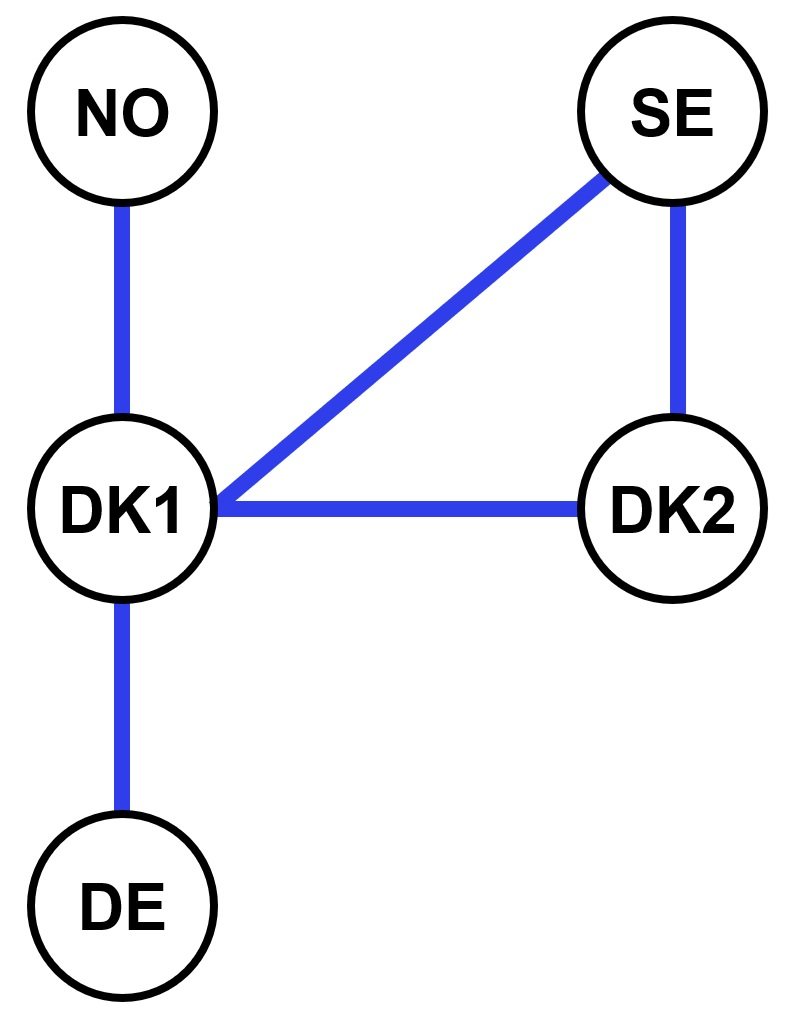
\includegraphics[width=0.2\linewidth]{figures/nodes.jpg}
    \caption{Simplified network.}
    \label{fig_network}
\end{figure}
\begin{itemize}
\item[a)] Create a list of the nodes and links. Sort the nodes and links in ascending order. Link (0,1) before (1,2), before (1,3) etc.
\item[b)] Calculate the degree of each node $k_i$  and the average degree of the network 〈k〉. 
\item[c)] Create the degree matrix $D_{ij}$. Create the adjacency matrix $A_{ij}$ and check that it is symmetric. 
\item[d)] Create the incidence matrix $K_{ij}$, assuming the links are always directed from low-number node to high-number node.
\item[e)] Create the Laplacian matrix $L_{ij}$  using the degree and adjacency matrices. Create the Laplacian matrix using the incidence matrix. Check that the two definitions agree. 
\end{itemize}

\end{problem}

\

\begin{problem}{3.3}
Using the Python package \href{https://networkx.org/}{networkX}, codify the network described in Problem 3.2. 

\begin{itemize}
\item[a)] Make a plot of the network.
\item[b)] Calculate the degree in every node and the average degree.
\item[c)] Calculate the Degree, Adjacency, Incidence and Laplacian matrix. Make a heat map of each of those matrices to evaluate them visually.

\end{itemize}

\textit{Hint: It is recommended to follow the} \href{https://martavp.github.io/integrated-energy-grids/intro-networkx.html#}{networkX tutorial} \textit{before trying this problem.}
\end{problem}

\

\begin{problem}{3.4}

In this problem, we will evaluate the transmission grid in Europe using data from ENTSOE and the Python package \href{https://networkx.org/}{networkX}.

\

Using the simplified dataset of the European high-voltage transmission network whose data is contained in the files 'data/nodes.csv' and 'data/edges.csv':

\begin{itemize}
\item[a)] Create a network object using 
 
\begin{verbatim}
nx.from_pandas_edgelist()
\end{verbatim}

and calculate the average degree.

\item[b)]  Add the information on the position of each node provided in 'data/nodes.csv' and make a plot of the network.

\item[c)]  Determine how many independent networks exist (these are the synchronous zones of the European transmission network).

\item[d)]  For the synchronous zone corresponding to Scandinavia, calculate the number of nodes and edges. Calculate the Degree, Adjacency, Incidence, and Laplacian matrices. Make a heat map of each of those matrices to evaluate them visually.

\end{itemize}

\end{problem}

%\begin{proof}[Solution]
%Write a solution here
%\end{proof}

\end{document}


 

